% !TEX program = pdflatex
% !TEX options = -synctex=1 -interaction=nonstopmode -file-line-error -shell-escape "%DOC%"

% \documentclass[crop,tikz,multi=false]{standalone}
\documentclass[crop,tikz,convert={outext=.svg,command=\unexpanded{pdf2svg \infile\space\outfile}},multi=false]{standalone}
\usetikzlibrary{shapes,backgrounds,decorations.pathreplacing,positioning}
\usepackage{amsfonts,amssymb,amsthm,amsmath}

\definecolor{mycolor1}{RGB}{27,158,119}
\definecolor{mycolor2}{RGB}{217,95,2}
\definecolor{mycolor3}{RGB}{117,112,179}

\tikzset{
    position/.style args={#1:#2 from #3}{
        at=(#3.#1), anchor=#1+180, shift=(#1:#2)
    }
}
\definecolor{mycolor1}{RGB}{27,158,119}
\definecolor{mycolor2}{RGB}{217,95,2}
\definecolor{mycolor3}{RGB}{117,112,179}
\begin{document}
\begin{tikzpicture}
    \tikzstyle{every node}=[font=\Large]

    \node[inner sep=0pt] (Figure0) at (0,0)
    {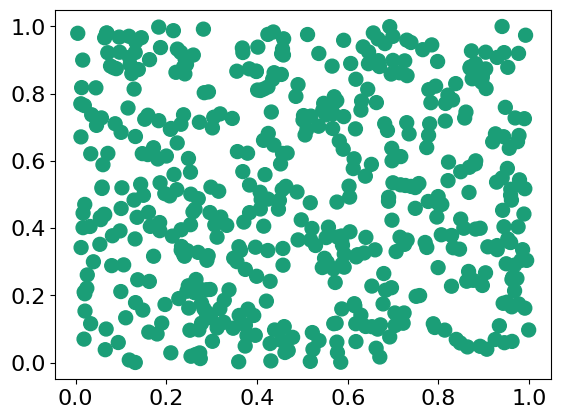
\includegraphics[width=.75\textwidth]{figure_0.png}};

    \node[inner sep=0pt] (Figure0) at (10,0)
    {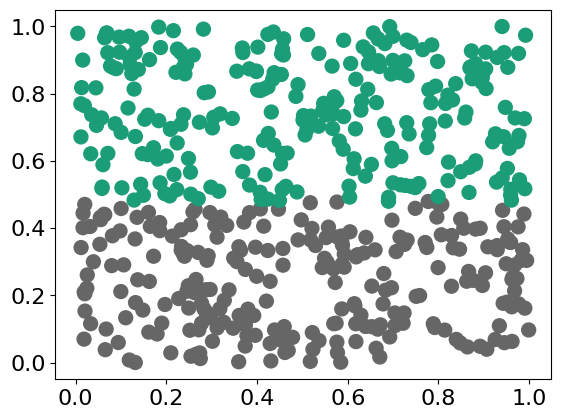
\includegraphics[width=.75\textwidth]{figure_1.png}};

    \node[inner sep=0pt] (Figure0) at (20,0)
    {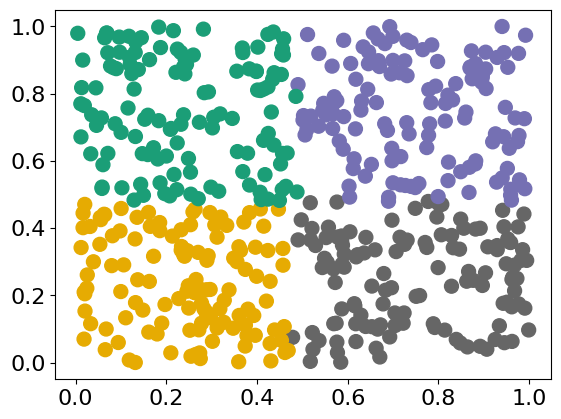
\includegraphics[width=.75\textwidth]{figure_2.png}};

    % Source tree
    \node[circle, draw=mycolor2, very thick, inner sep=1pt] at (0.4,-5) (Is00) {\(Cl^{(0)}_1\)} ;
    \node[position=-140:1 from Is00] (Is10) {\(Cl^{(1)}_1\)} ;
    \node[position=-40:1 from Is00] (Is11) {\(Cl^{(1)}_2\)} ;
    \node[position=-120:1 from Is10] (Is20) {\(Cl^{(2)}_1\)} ;
    \node[position=-60:1 from Is10] (Is21) {\(Cl^{(2)}_2\)} ;
    \node[position=-120:1 from Is11] (Is22) {\(Cl^{(2)}_3\)} ;
    \node[position=-60:1 from Is11] (Is23) {\(Cl^{(2)}_4\)} ;

    \draw (Is00) -- (Is10);
    \draw (Is00) -- (Is11);
    \draw (Is10) -- (Is20);
    \draw (Is10) -- (Is21);
    \draw (Is11) -- (Is22);
    \draw (Is11) -- (Is23);

    % Source tree
    \node at (10.4,-5) (Is00) {\(Cl^{(0)}_1\)} ;
    \node[circle, draw=mycolor2, very thick, inner sep=1pt, position=-140:1 from Is00] (Is10) {\(Cl^{(1)}_1\)} ;
    \node[circle, draw=mycolor2, very thick, inner sep=1pt, position=-40:1 from Is00] (Is11) {\(Cl^{(1)}_2\)} ;
    \node[position=-120:1 from Is10] (Is20) {\(Cl^{(2)}_1\)} ;
    \node[position=-60:1 from Is10] (Is21) {\(Cl^{(2)}_2\)} ;
    \node[position=-120:1 from Is11] (Is22) {\(Cl^{(2)}_3\)} ;
    \node[position=-60:1 from Is11] (Is23) {\(Cl^{(2)}_4\)} ;

    \draw (Is00) -- (Is10);
    \draw (Is00) -- (Is11);
    \draw (Is10) -- (Is20);
    \draw (Is10) -- (Is21);
    \draw (Is11) -- (Is22);
    \draw (Is11) -- (Is23);


    % Source tree
    \node at (20.4,-5) (Is00) {\(Cl^{(0)}_1\)} ;
    \node[position=-140:1 from Is00] (Is10) {\(Cl^{(1)}_1\)} ;
    \node[position=-40:1 from Is00] (Is11) {\(Cl^{(1)}_2\)} ;
    \node[circle, draw=mycolor2, very thick, inner sep=1pt, position=-120:1 from Is10] (Is20) {\(Cl^{(2)}_1\)} ;
    \node[circle, draw=mycolor2, very thick, inner sep=1pt, position=-60:1 from Is10] (Is21) {\(Cl^{(2)}_2\)} ;
    \node[circle, draw=mycolor2, very thick, inner sep=1pt, position=-120:1 from Is11] (Is22) {\(Cl^{(2)}_3\)} ;
    \node[circle, draw=mycolor2, very thick, inner sep=1pt, position=-60:1 from Is11] (Is23) {\(Cl^{(2)}_4\)} ;

    \draw (Is00) -- (Is10);
    \draw (Is00) -- (Is11);
    \draw (Is10) -- (Is20);
    \draw (Is10) -- (Is21);
    \draw (Is11) -- (Is22);
    \draw (Is11) -- (Is23);



\end{tikzpicture}
\end{document}
